\documentclass[dvisvgm]{standalone}

\usepackage{tikz}
\usetikzlibrary {arrows.meta, positioning, automata}

\begin{document}

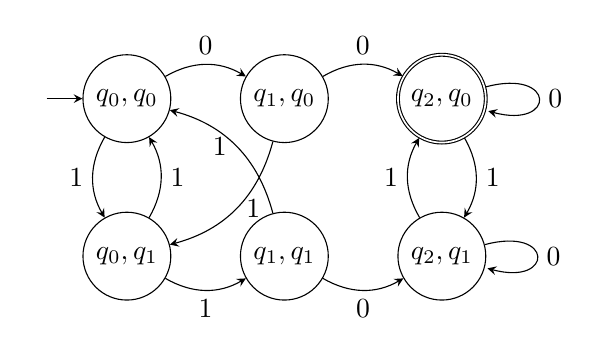
\begin{tikzpicture}[
    ->,
    >=stealth,
    node distance=2cm,
    initial text=$ $,
    on grid,
]

    \node[initial,   state]              (A) {$q_0, q_0$};
    \node[           state, right =of A] (B) {$q_1, q_0$};
    \node[accepting, state, right =of B] (C) {$q_2, q_0$};
    \node[           state, below =of A] (D) {$q_0, q_1$};
    \node[           state, right =of D] (E) {$q_1, q_1$};
    \node[           state, right =of E] (F) {$q_2, q_1$};

    \path
        (A) edge [bend left, above]  node {0}     (B)
        (B) edge [bend left, above]  node {0}     (C)
        (C) edge [loop right]        node {0}     (C)
        (C) edge [bend left, right]  node {1}     (F)
        (F) edge [bend left,  left]  node {1}     (C)
        (F) edge [loop right]        node {0}     (F)
        (E) edge [bend right, below] node {0}     (F)
        (D) edge [bend right, below] node {1}     (E)
        (A) edge [bend right,  left] node {1}     (D)
        (D) edge [bend right, right] node {1}     (A)
        (E) edge [bend right,  left] node {1}     (A)
        (B) edge [bend left,  right] node {1}     (D)
    ;
\end{tikzpicture}

\end{document}